\documentclass[10pt,a4paper]{article}

% Standalone manuscript-style subsection that can be compiled directly
% or adapted into a larger PLOS Computational Biology manuscript.

\usepackage[margin=1in]{geometry}
\usepackage[british]{babel}
\usepackage[T1]{fontenc}
\usepackage[utf8]{inputenc}
\usepackage{microtype}
\usepackage{setspace}
\usepackage{mathtools,amssymb}
\usepackage{graphicx}
\usepackage{natbib}
\usepackage[hidelinks]{hyperref}

\onehalfspacing

\begin{document}

\section*{Methods}
\subsection*{Model overview}

For each sampled pair of cases $i$ and $j$, \texttt{EpiLink} evaluates whether the observed testing-time difference and consensus-level genetic distance are compatible with a finite set of recent latent transmission histories. Let
\begin{align}
t_{ij} = t_{\mathrm{test},j} - t_{\mathrm{test},i}
\end{align}
denote the observed difference in testing times, and let $g_{ij}$ denote the observed consensus-level genetic distance. Candidate latent histories are drawn from
\begin{align}
\mathcal{S}_M
=
\left\{
H_{\mathrm{AD}}(m): m=0,\ldots,M
\right\}
\cup
\left\{
H_{\mathrm{CA}}(m_i,m_j): m_i,m_j \ge 0,\ m_i+m_j \le M
\right\}.
\end{align}
Here, $H_{\mathrm{AD}}(m)$ is an ancestor--descendant history with $m$ unsampled intermediates, and $H_{\mathrm{CA}}(m_i,m_j)$ is a common-ancestor history in which the two sampled cases descend from a shared unsampled source with branch depths $m_i$ and $m_j$. Direct transmission and co-primary infection are recovered as the special cases $H_{\mathrm{AD}}(0)$ and $H_{\mathrm{CA}}(0,0)$, respectively (Fig.~\ref{fig:latent_histories}).

\begin{figure}[ht]
\centering
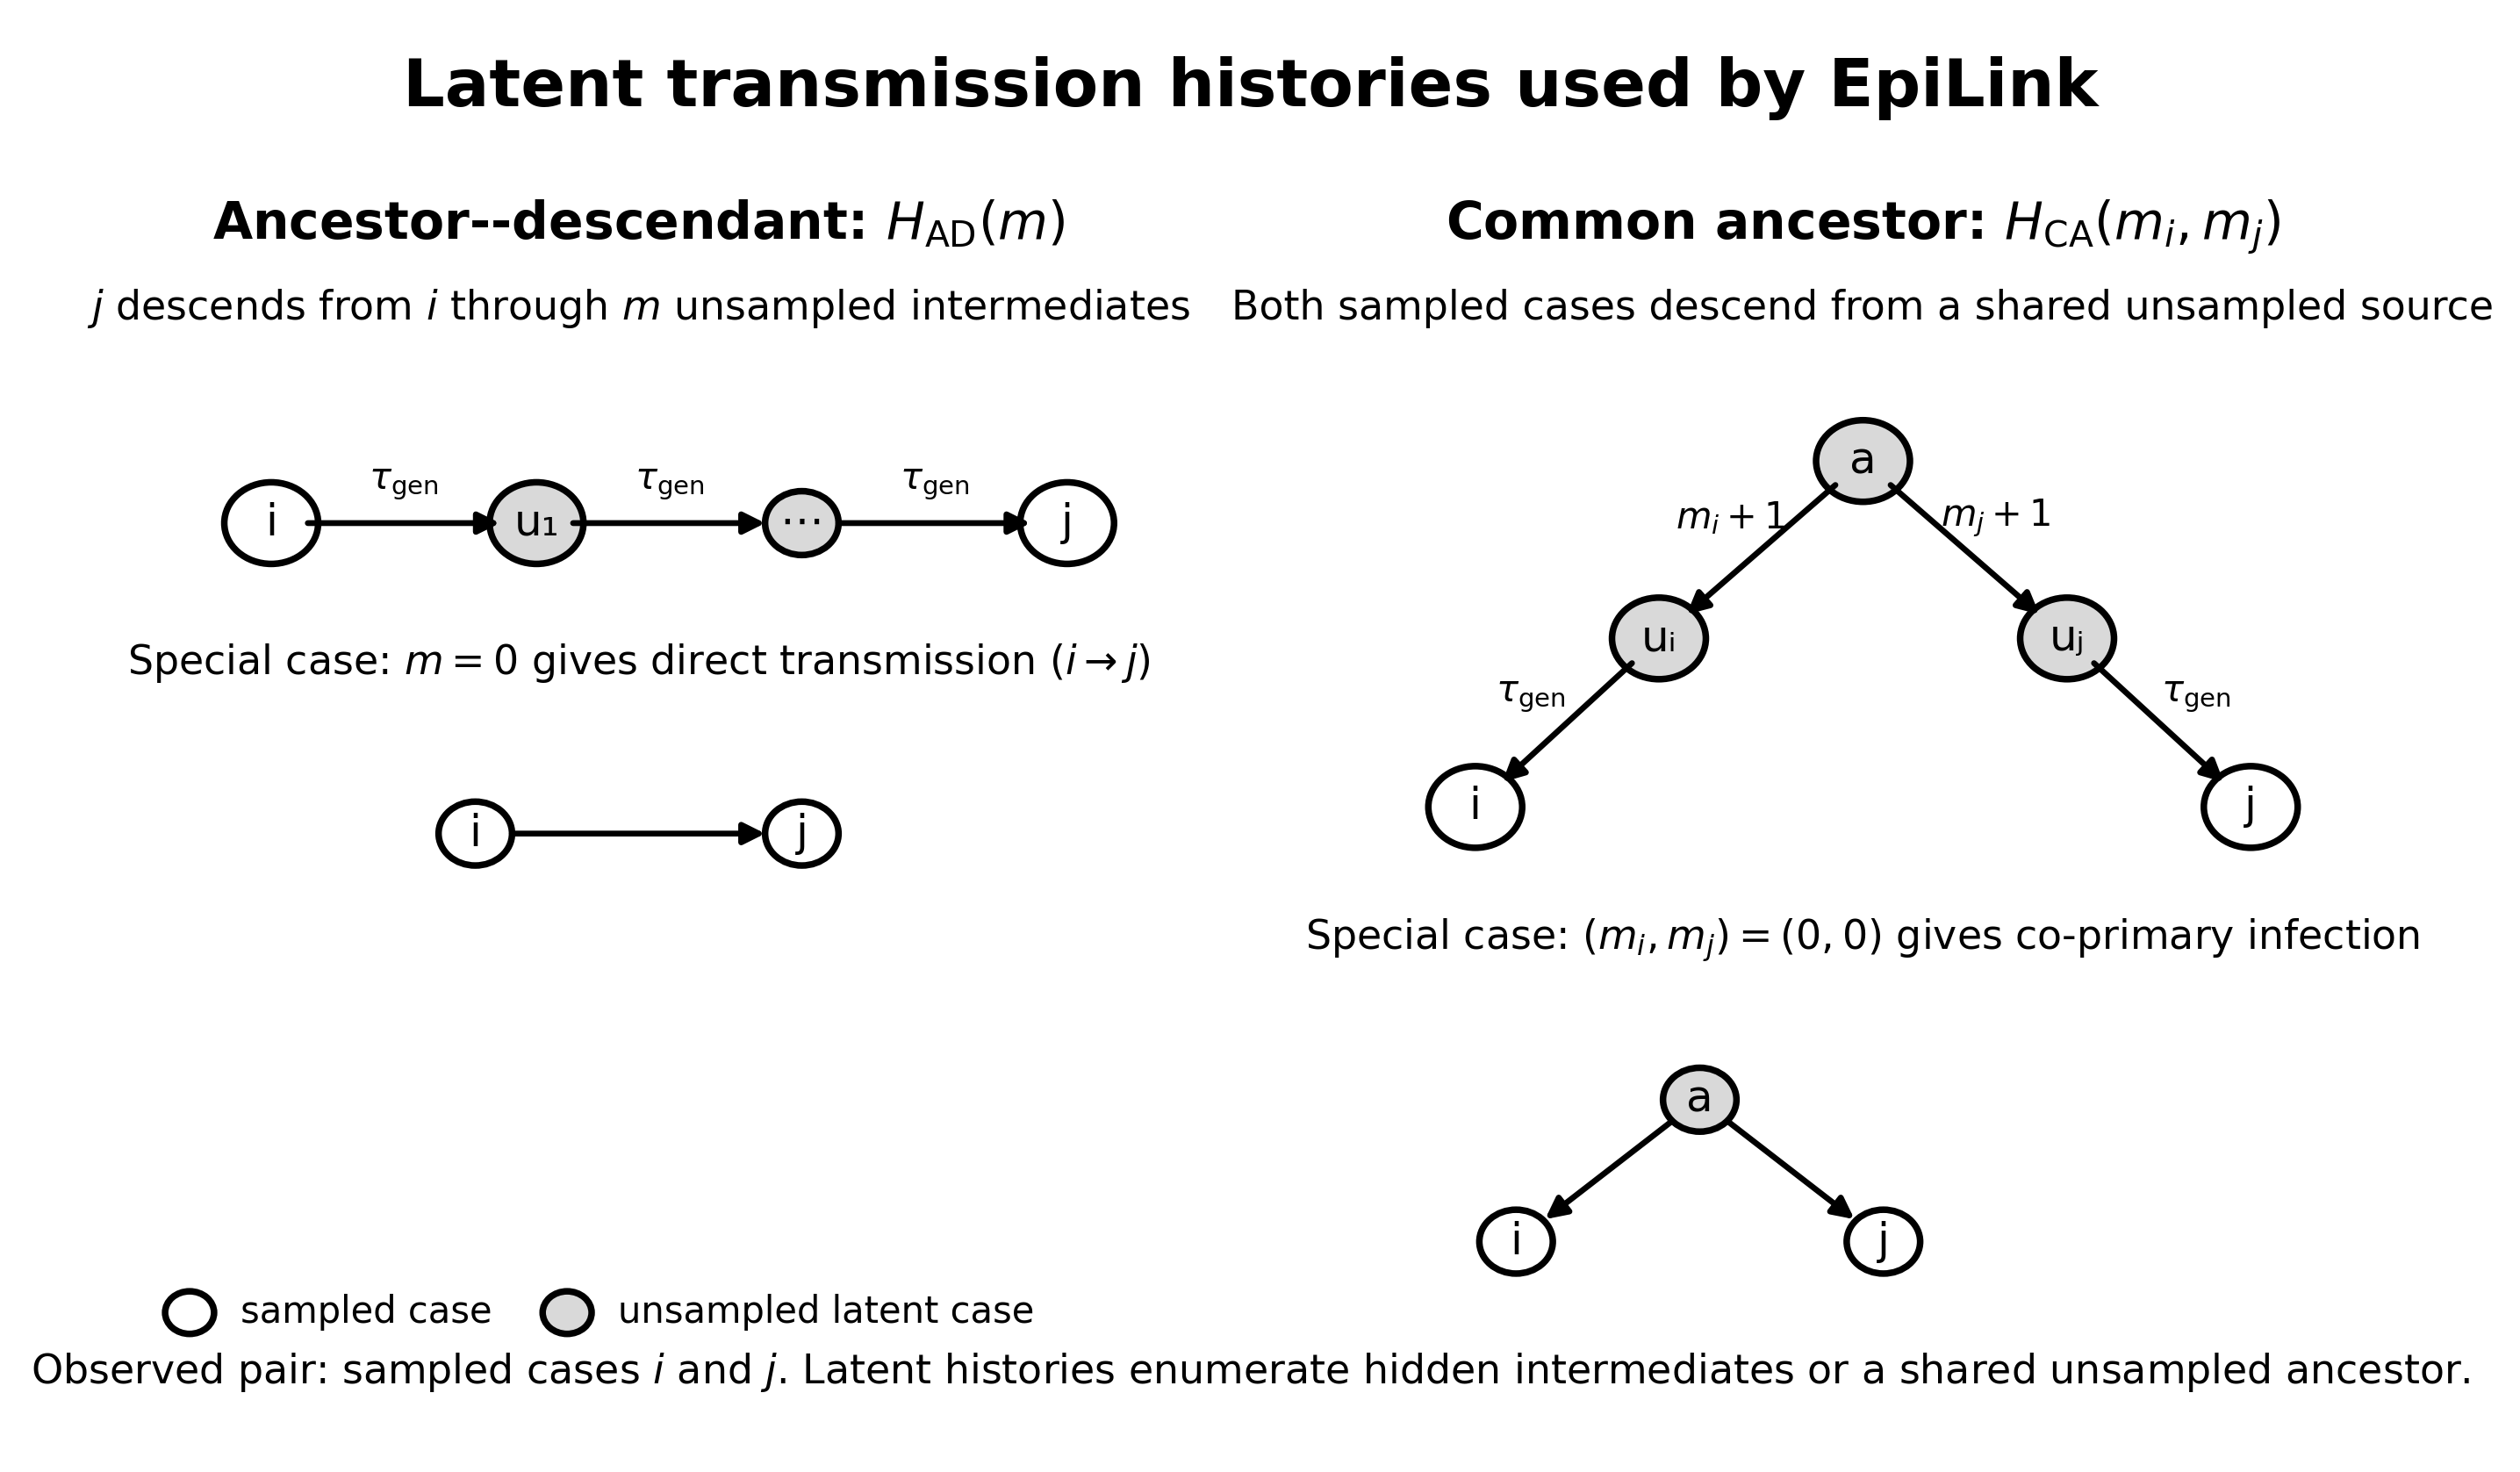
\includegraphics[width=0.95\linewidth]{epilink_scenarios}
\caption{\textbf{Latent transmission histories considered by \texttt{EpiLink}.} Schematic representation of the two families of latent transmission histories linking a sampled pair of cases $i$ and $j$. In the ancestor--descendant history $H_{\mathrm{AD}}(m)$, case $j$ descends from case $i$ through $m$ unsampled intermediates; the special case $m=0$ corresponds to direct transmission. In the common-ancestor history $H_{\mathrm{CA}}(m_i,m_j)$, both sampled cases descend from a shared unsampled source, with branch depths $m_i$ and $m_j$; the special case $(m_i,m_j)=(0,0)$ corresponds to co-primary infection. Open circles denote sampled cases and shaded circles denote unsampled latent cases. These latent histories define the scenario set over which temporal and genetic compatibility scores are evaluated.}
\label{fig:latent_histories}
\end{figure}

The temporal component is based on an $E/P/I$ infection-process model with Gamma-distributed latent, presymptomatic infectious, and symptomatic infectious stages \citep{Hart2021}, together with a Gamma-distributed delay from symptom onset to testing. Writing $\tau_{\mathrm{inc}} = y_E + y_P$ for the incubation period and $\tau_{\mathrm{gen}} = \tau_{\mathrm{inc}} + y_{\mathrm{toit}}$ for the generation interval, the model-implied testing-time difference under scenario $s$ is
\begin{align}
T_s
=
A_j(s) - A_i(s)
+
\tau_{\mathrm{inc},j} + x_{\mathrm{test},j}
-
\tau_{\mathrm{inc},i} - x_{\mathrm{test},i},
\end{align}
where $A_k(s)$ is the elapsed time from the latent reference point to infection of sampled case $k$. Under an ancestor--descendant history,
\begin{align}
A_i\!\left(H_{\mathrm{AD}}(m)\right) &= 0,\\
A_j\!\left(H_{\mathrm{AD}}(m)\right) &= \sum_{r=0}^{m}\tau_{\mathrm{gen},r},
\end{align}
so that
\begin{align}
T_{ij}\!\left(H_{\mathrm{AD}}(m)\right)
=
\sum_{r=0}^{m}\tau_{\mathrm{gen},r}
+
\tau_{\mathrm{inc},j} + x_{\mathrm{test},j}
-
\tau_{\mathrm{inc},i} - x_{\mathrm{test},i}.
\end{align}
Under a common-ancestor history,
\begin{align}
A_i\!\left(H_{\mathrm{CA}}(m_i,m_j)\right)
&=
\sum_{r=1}^{m_i+1}\tau_{\mathrm{gen},r}^{(i)},\\
A_j\!\left(H_{\mathrm{CA}}(m_i,m_j)\right)
&=
\sum_{s=1}^{m_j+1}\tau_{\mathrm{gen},s}^{(j)},
\end{align}
giving
\begin{align}
T_{ij}\!\left(H_{\mathrm{CA}}(m_i,m_j)\right)
=
\sum_{s=1}^{m_j+1}\tau_{\mathrm{gen},s}^{(j)}
-
\sum_{r=1}^{m_i+1}\tau_{\mathrm{gen},r}^{(i)}
+
\tau_{\mathrm{inc},j} + x_{\mathrm{test},j}
-
\tau_{\mathrm{inc},i} - x_{\mathrm{test},i}.
\end{align}
For each scenario, Monte Carlo simulation yields draws from the induced temporal distribution.

The genetic component assumes that within-host divergence is negligible on the timescales of interest and that consensus divergence accumulates along transmission-linked lineages. Let $B_s$ denote the effective transmission-related branch length under scenario $s$. For ancestor--descendant histories,
\begin{align}
B_{ij}\!\left(H_{\mathrm{AD}}(m)\right)
=
\sum_{r=0}^{m}\tau_{\mathrm{gen},r}
+
\tau_{\mathrm{inc},j} + x_{\mathrm{test},j}
-
\bigl(\tau_{\mathrm{inc},i} + x_{\mathrm{test},i}\bigr),
\end{align}
whereas for common-ancestor histories,
\begin{align}
B_{ij}\!\left(H_{\mathrm{CA}}(m_i,m_j)\right)
=
\sum_{r=1}^{m_i+1}\tau_{\mathrm{gen},r}^{(i)}
+
\sum_{s=1}^{m_j+1}\tau_{\mathrm{gen},s}^{(j)}
+
\tau_{\mathrm{inc},i} + x_{\mathrm{test},i}
+
\tau_{\mathrm{inc},j} + x_{\mathrm{test},j}.
\end{align}
If $r$ is the median substitution rate per site per year and $L$ is genome length, then the corresponding per-genome daily rate is
\begin{align}
\lambda = \frac{rL}{365}.
\end{align}
Given branch-length draw $B_s^{(n)}$, the expected genetic draw is
\begin{align}
G_s^{(n)} = \lambda B_s^{(n)},
\end{align}
or, under a stochastic mutational process,
\begin{align}
G_s^{(n)} \mid B_s^{(n)},\lambda
\sim
\mathrm{Poisson}\!\left(\lambda B_s^{(n)}\right).
\end{align}

A relaxed uncorrelated log-normal clock can be used by drawing $r^{(n)}$ and replacing $\lambda$ with $\lambda^{(n)} = r^{(n)}L/365$.

Observed temporal and genetic distances are scored against the simulated scenario-specific distributions using percentile-based compatibility measures. For any observed quantity $x_{\mathrm{obs}}$ and scenario-specific Monte Carlo draws $x_1^{(s)},\ldots,x_{n_s}^{(s)}$, define
\begin{align}
p_s(x_{\mathrm{obs}})
=
\frac{\#\left\{i:x_i^{(s)} \le x_{\mathrm{obs}}\right\}}{n_s},
\qquad
C_s(x_{\mathrm{obs}})
=
1 - 2\left|p_s(x_{\mathrm{obs}}) - 0.5\right|.
\end{align}
Applying this separately to the temporal and genetic components yields $C_{T,s}(i,j)$ and $C_{G,s}(i,j)$, and the overall compatibility for scenario $s$ is
\begin{align}
C_s(i,j) = C_{T,s}(i,j)\,C_{G,s}(i,j).
\end{align}
To represent broader hypotheses, scores may then be summed across any user-defined target subset $\mathcal{S}_\star \subseteq \mathcal{S}_M$:
\begin{align}
\mathrm{score}_{\mathcal{S}_\star}(i,j)
=
\sum_{s \in \mathcal{S}_\star} C_s(i,j).
\end{align}
Because scenario-specific temporal and genetic draws are precomputed and cached, pairwise evaluation requires only percentile lookups against stored Monte Carlo samples, making the method scalable to large datasets.

\bibliographystyle{plainnat}
\bibliography{references}

\end{document}
